
%% bare_conf.tex
%% V1.4b
%% 2015/08/26
%% by Michael Shell
%% See:
%% http://www.michaelshell.org/
%% for current contact information.
%%
%% This is a skeleton file demonstrating the use of IEEEtran.cls
%% (requires IEEEtran.cls version 1.8b or later) with an IEEE
%% conference paper.
%%
%% Support sites:
%% http://www.michaelshell.org/tex/ieeetran/
%% http://www.ctan.org/pkg/ieeetran
%% and
%% http://www.ieee.org/

%%*************************************************************************
%% Legal Notice:
%% This code is offered as-is without any warranty either expressed or
%% implied; without even the implied warranty of MERCHANTABILITY or
%% FITNESS FOR A PARTICULAR PURPOSE! 
%% User assumes all risk.
%% In no event shall the IEEE or any contributor to this code be liable for
%% any damages or losses, including, but not limited to, incidental,
%% consequential, or any other damages, resulting from the use or misuse
%% of any information contained here.
%%
%% All comments are the opinions of their respective authors and are not
%% necessarily endorsed by the IEEE.
%%
%% This work is distributed under the LaTeX Project Public License (LPPL)
%% ( http://www.latex-project.org/ ) version 1.3, and may be freely used,
%% distributed and modified. A copy of the LPPL, version 1.3, is included
%% in the base LaTeX documentation of all distributions of LaTeX released
%% 2003/12/01 or later.
%% Retain all contribution notices and credits.
%% ** Modified files should be clearly indicated as such, including  **
%% ** renaming them and changing author support contact information. **
%%*************************************************************************


% *** Authors should verify (and, if needed, correct) their LaTeX system  ***
% *** with the testflow diagnostic prior to trusting their LaTeX platform ***
% *** with production work. The IEEE's font choices and paper sizes can   ***
% *** trigger bugs that do not appear when using other class files.       ***                          ***
% The testflow support page is at:
% http://www.michaelshell.org/tex/testflow/



\documentclass[conference]{IEEEtran}
% Some Computer Society conferences also require the compsoc mode option,
% but others use the standard conference format.
%
% If IEEEtran.cls has not been installed into the LaTeX system files,
% manually specify the path to it like:
% \documentclass[conference]{../sty/IEEEtran}





% Some very useful LaTeX packages include:
% (uncomment the ones you want to load)


% *** MISC UTILITY PACKAGES ***
%
%\usepackage{ifpdf}
% Heiko Oberdiek's ifpdf.sty is very useful if you need conditional
% compilation based on whether the output is pdf or dvi.
% usage:
% \ifpdf
%   % pdf code
% \else
%   % dvi code
% \fi
% The latest version of ifpdf.sty can be obtained from:
% http://www.ctan.org/pkg/ifpdf
% Also, note that IEEEtran.cls V1.7 and later provides a builtin
% \ifCLASSINFOpdf conditional that works the same way.
% When switching from latex to pdflatex and vice-versa, the compiler may
% have to be run twice to clear warning/error messages.






% *** CITATION PACKAGES ***
%
\usepackage{cite}
% cite.sty was written by Donald Arseneau
% V1.6 and later of IEEEtran pre-defines the format of the cite.sty package
% \cite{} output to follow that of the IEEE. Loading the cite package will
% result in citation numbers being automatically sorted and properly
% "compressed/ranged". e.g., [1], [9], [2], [7], [5], [6] without using
% cite.sty will become [1], [2], [5]--[7], [9] using cite.sty. cite.sty's
% \cite will automatically add leading space, if needed. Use cite.sty's
% noadjust option (cite.sty V3.8 and later) if you want to turn this off
% such as if a citation ever needs to be enclosed in parenthesis.
% cite.sty is already installed on most LaTeX systems. Be sure and use
% version 5.0 (2009-03-20) and later if using hyperref.sty.
% The latest version can be obtained at:
% http://www.ctan.org/pkg/cite
% The documentation is contained in the cite.sty file itself.






% *** GRAPHICS RELATED PACKAGES ***
%
\ifCLASSINFOpdf
   \usepackage[pdftex]{graphicx}
  % declare the path(s) where your graphic files are
   \graphicspath{{g/}}
  % and their extensions so you won't have to specify these with
  % every instance of \includegraphics
  \DeclareGraphicsExtensions{.pdf,.jpeg,.png,.PNG}
\else
  % or other class option (dvipsone, dvipdf, if not using dvips). graphicx
  % will default to the driver specified in the system graphics.cfg if no
  % driver is specified.
  % \usepackage[dvips]{graphicx}
  % declare the path(s) where your graphic files are
  % \graphicspath{{../eps/}}
  % and their extensions so you won't have to specify these with
  % every instance of \includegraphics
  % \DeclareGraphicsExtensions{.eps}
\fi
% graphicx was written by David Carlisle and Sebastian Rahtz. It is
% required if you want graphics, photos, etc. graphicx.sty is already
% installed on most LaTeX systems. The latest version and documentation
% can be obtained at: 
% http://www.ctan.org/pkg/graphicx
% Another good source of documentation is "Using Imported Graphics in
% LaTeX2e" by Keith Reckdahl which can be found at:
% http://www.ctan.org/pkg/epslatex
%
% latex, and pdflatex in dvi mode, support graphics in encapsulated
% postscript (.eps) format. pdflatex in pdf mode supports graphics
% in .pdf, .jpeg, .png and .mps (metapost) formats. Users should ensure
% that all non-photo figures use a vector format (.eps, .pdf, .mps) and
% not a bitmapped formats (.jpeg, .png). The IEEE frowns on bitmapped formats
% which can result in "jaggedy"/blurry rendering of lines and letters as
% well as large increases in file sizes.
%
% You can find documentation about the pdfTeX application at:
% http://www.tug.org/applications/pdftex





% *** MATH PACKAGES ***
%
%\usepackage{amsmath}
% A popular package from the American Mathematical Society that provides
% many useful and powerful commands for dealing with mathematics.
%
% Note that the amsmath package sets \interdisplaylinepenalty to 10000
% thus preventing page breaks from occurring within multiline equations. Use:
%\interdisplaylinepenalty=2500
% after loading amsmath to restore such page breaks as IEEEtran.cls normally
% does. amsmath.sty is already installed on most LaTeX systems. The latest
% version and documentation can be obtained at:
% http://www.ctan.org/pkg/amsmath





% *** SPECIALIZED LIST PACKAGES ***
%
%\usepackage{algorithmic}
% algorithmic.sty was written by Peter Williams and Rogerio Brito.
% This package provides an algorithmic environment fo describing algorithms.
% You can use the algorithmic environment in-text or within a figure
% environment to provide for a floating algorithm. Do NOT use the algorithm
% floating environment provided by algorithm.sty (by the same authors) or
% algorithm2e.sty (by Christophe Fiorio) as the IEEE does not use dedicated
% algorithm float types and packages that provide these will not provide
% correct IEEE style captions. The latest version and documentation of
% algorithmic.sty can be obtained at:
% http://www.ctan.org/pkg/algorithms
% Also of interest may be the (relatively newer and more customizable)
% algorithmicx.sty package by Szasz Janos:
% http://www.ctan.org/pkg/algorithmicx




% *** ALIGNMENT PACKAGES ***
%
%\usepackage{array}
% Frank Mittelbach's and David Carlisle's array.sty patches and improves
% the standard LaTeX2e array and tabular environments to provide better
% appearance and additional user controls. As the default LaTeX2e table
% generation code is lacking to the point of almost being broken with
% respect to the quality of the end results, all users are strongly
% advised to use an enhanced (at the very least that provided by array.sty)
% set of table tools. array.sty is already installed on most systems. The
% latest version and documentation can be obtained at:
% http://www.ctan.org/pkg/array


% IEEEtran contains the IEEEeqnarray family of commands that can be used to
% generate multiline equations as well as matrices, tables, etc., of high
% quality.




% *** SUBFIGURE PACKAGES ***
%\ifCLASSOPTIONcompsoc
%  \usepackage[caption=false,font=normalsize,labelfont=sf,textfont=sf]{subfig}
%\else
%  \usepackage[caption=false,font=footnotesize]{subfig}
%\fi
% subfig.sty, written by Steven Douglas Cochran, is the modern replacement
% for subfigure.sty, the latter of which is no longer maintained and is
% incompatible with some LaTeX packages including fixltx2e. However,
% subfig.sty requires and automatically loads Axel Sommerfeldt's caption.sty
% which will override IEEEtran.cls' handling of captions and this will result
% in non-IEEE style figure/table captions. To prevent this problem, be sure
% and invoke subfig.sty's "caption=false" package option (available since
% subfig.sty version 1.3, 2005/06/28) as this is will preserve IEEEtran.cls
% handling of captions.
% Note that the Computer Society format requires a larger sans serif font
% than the serif footnote size font used in traditional IEEE formatting
% and thus the need to invoke different subfig.sty package options depending
% on whether compsoc mode has been enabled.
%
% The latest version and documentation of subfig.sty can be obtained at:
% http://www.ctan.org/pkg/subfig




% *** FLOAT PACKAGES ***



%\usepackage{stfloats}
% stfloats.sty was written by Sigitas Tolusis. This package gives LaTeX2e
% the ability to do double column floats at the bottom of the page as well
% as the top. (e.g., "\begin{figure*}[!b]" is not normally possible in
% LaTeX2e). It also provides a command:
%\fnbelowfloat
% to enable the placement of footnotes below bottom floats (the standard
% LaTeX2e kernel puts them above bottom floats). This is an invasive package
% which rewrites many portions of the LaTeX2e float routines. It may not work
% with other packages that modify the LaTeX2e float routines. The latest
% version and documentation can be obtained at:
% http://www.ctan.org/pkg/stfloats
% Do not use the stfloats baselinefloat ability as the IEEE does not allow
% \baselineskip to stretch. Authors submitting work to the IEEE should note
% that the IEEE rarely uses double column equations and that authors should try
% to avoid such use. Do not be tempted to use the cuted.sty or midfloat.sty
% packages (also by Sigitas Tolusis) as the IEEE does not format its papers in
% such ways.
% Do not attempt to use stfloats with fixltx2e as they are incompatible.
% Instead, use Morten Hogholm'a dblfloatfix which combines the features
% of both fixltx2e and stfloats:
%
% \usepackage{dblfloatfix}
% The latest version can be found at:
% http://www.ctan.org/pkg/dblfloatfix




% *** PDF, URL AND HYPERLINK PACKAGES ***
%
%\usepackage{url}
% url.sty was written by Donald Arseneau. It provides better support for
% handling and breaking URLs. url.sty is already installed on most LaTeX
% systems. The latest version and documentation can be obtained at:
% http://www.ctan.org/pkg/url
% Basically, \url{my_url_here}.




% *** Do not adjust lengths that control margins, column widths, etc. ***
% *** Do not use packages that alter fonts (such as pslatex).         ***
% There should be no need to do such things with IEEEtran.cls V1.6 and later.
% (Unless specifically asked to do so by the journal or conference you plan
% to submit to, of course. )


% correct bad hyphenation here
\hyphenation{op-tical net-works semi-conduc-tor}


\begin{document}
%
% paper title
% Titles are generally capitalized except for words such as a, an, and, as,
% at, but, by, for, in, nor, of, on, or, the, to and up, which are usually
% not capitalized unless they are the first or last word of the title.
% Linebreaks \\ can be used within to get better formatting as desired.
% Do not put math or special symbols in the title.
\title{Making Matches - Recommending the Right Personalities}


% author names and affiliations
% use a multiple column layout for up to three different
% affiliations
\author{\IEEEauthorblockN{Paul Schweiger}
\IEEEauthorblockA{2103468\\
	Multimedia Seminar II\\
Technische Universität Darmstadt}}

% conference papers do not typically use \thanks and this command
% is locked out in conference mode. If really needed, such as for
% the acknowledgment of grants, issue a \IEEEoverridecommandlockouts
% after \documentclass

% for over three affiliations, or if they all won't fit within the width
% of the page, use this alternative format:
% 
%\author{\IEEEauthorblockN{Michael Shell\IEEEauthorrefmark{1},
%Homer Simpson\IEEEauthorrefmark{2},
%James Kirk\IEEEauthorrefmark{3}, 
%Montgomery Scott\IEEEauthorrefmark{3} and
%Eldon Tyrell\IEEEauthorrefmark{4}}
%\IEEEauthorblockA{\IEEEauthorrefmark{1}School of Electrical and Computer Engineering\\
%Georgia Institute of Technology,
%Atlanta, Georgia 30332--0250\\ Email: see http://www.michaelshell.org/contact.html}
%\IEEEauthorblockA{\IEEEauthorrefmark{2}Twentieth Century Fox, Springfield, USA\\
%Email: homer@thesimpsons.com}
%\IEEEauthorblockA{\IEEEauthorrefmark{3}Starfleet Academy, San Francisco, California 96678-2391\\
%Telephone: (800) 555--1212, Fax: (888) 555--1212}
%\IEEEauthorblockA{\IEEEauthorrefmark{4}Tyrell Inc., 123 Replicant Street, Los Angeles, California 90210--4321}}




% use for special paper notices
%\IEEEspecialpapernotice{(Invited Paper)}




% make the title area
\maketitle

% As a general rule, do not put math, special symbols or citations
% in the abstract
\begin{abstract}
Recommender Systems can be used to guide our limited time and attention towards meaningful actions, items, content or people. To tailor results to a user, Recommender Systems need to account for a user's preferences, skills and personality and incorporate these into a unified user model. These models need to be descriptive without overcomplicating the system. In social situations such as learning, recommendations become more complicated, as several users and their respective models need to be combined. Reciprocal recommendations can improve the quality of matchups by ensuring a good fit and benefit for both parties.\\
A recent approach to implement a reciprocal peer recommendation platform for learning purposes by Potts et al. aims to show how these theories can be used in praxis. \cite{potts2018reciprocal} The system enables students to find study-partners of matching skill for different learning topics by reciprocally recommending them to each other according to their respective preferences.\\
Based on this study, the intricacies of proper user modeling, reciprocal recommendations and researching new algorithms are highlighted. Common issues include unreliable self-reported user data, unevaluated algorithms and unfitting user models. Successful systems need to incorporate both explicit and implicit user feedback. Proper theoretical founding and preliminary considerations can solidify and improve reciprocal Recommender Systems.\\
\end{abstract}

% no keywords


\IEEEpeerreviewmaketitle


\section{Introduction}
The modern world provides a plethora of opportunities, topics, people or products to consume, engage with or discuss, while people have a limited amount of attention and time to spend. As the offline world embraces online opportunities, this surplus of possible interactions is multiplied even further. In order to help us guide our attention and resources, basically every digital system tries to recommend meaningful content to users. Recommender Systems play a critical role in modern society and have transcended many different domains, pervading our lifes in advertising, e-learning, e-commerce, data analysis, online-dating, video game matchmaking, social networks, and others.\\
These highly unique topics make generalizing Recommender Systems difficult, leading to many different solutions for loosely related problems. \cite{BUDER2012207} Combining some of these approaches, common techniques regarding tasks such as user modeling or social recommendation become prevalent. Employing Recommender Systems in social environments, helping users to engage with the right person at the right time, becomes a possibility that could shape interactions between people in lots of domains.\\ 
While social contacts prove highly important in many aspects of life, social and cooperative learning are also known to positively affect learning outcomes. \cite{bossert1982instructional, blumenfeld1996learning} Successful group learning efforts can enhance cognitive and intellectual performance, student's social and communicative skills and influence their overall satisfaction. \cite{zhao2004adding, maxwell2008learning} Thus, social recommendation for learning is an important topic, helping to make mankind both more successful and happier at the same time.\\
To take advantage of social learning, research has diverted from the more traditional view of technology-enhanced learning, that focuses on improving individual learning experiences by recommending exercises, media resources or additional information at the right time depending on student's skills, preferences, needs and personality \cite{drachsler2015panorama, erdt2015evaluating}. Social learning research tries to connect learners to each other. Researchers have for example explored opportunities for students to receive immediate peer support via online requests \cite{greer1998intelligent} or tasked students to discuss their answers to exercises in an e-learning environment with peers, which led to improvements in both short- and long-term performance. \cite{reidsema2016exploring}\\
The goal of this report is to emphasize the importance and common problems of proper user modeling and preference management for reciprocal social recommendations, especially in a learning context. Such Recommender Systems can not only be used to help a single learner solve problems or improve learning results, but to connect people, to build a community of learners and to enable students to engage in meaningful social learning opportunities. Along the way, relevant examples from other domains will be featured. After a quick introduction into the basics of user modeling and social recommendations in section \ref{relatedwork}, section \ref{paper} will discuss a very recent paper by Potts et al. introducing a reciprocal Recommender System for learning environments. \cite{potts2018reciprocal} Finally, section \ref{extensions} will discuss the paper's proposed prototype and highlight some of the intricacies of reciprocal recommendation and learning group formation.\\

\section{Related Work: Recommender Systems} \label{relatedwork}

The goal of a Recommender System [RS] is to emphasize relevant pieces of information in a convoluted stream of data, and to recommend a specific result to a specific user based on his or her history, preferences and situation. \cite{ricci2011introduction}\\
The following sections outline relevant findings and concepts regarding Recommender Systems in social environments and reciprocal peer recommendation. We will take a look at the basics of user modeling, social recommendations and the importance of reciprocality.

\subsection{User Modeling} \label{rw:usermodeling}
In order to successfully recommend items, an RS needs to understand it's user. Goals, circumstances and domain-specific aspects need to be considered. Thus, RS need to model their users to try and understand what items might be relevant. Recommender Systems need to account for an adequate operationalization of the relevant personality traits, domain-specific preferences and surrounding circumstances and combine these into a user model.\\
Different domains or approaches within the same domain require different user models. For example, information about people connected to the current user can be helpful to improve recommendation quality. Based on user friendships and shared interests, specific items that one person liked could be recommended to friends \cite{feng2013recommendation} or just other users with comparable interests via implicit user connections. \cite{8328917} For example, a user's contacts and geographic history could be accessed to find users with matching profiles and to use their information to improve recommendations. \cite{ramaswamy2009caesar}\\ 
For example in competitive multiplayer gaming, which is currently gaining in importance due to the increased interest in e-sports, the main goal is to create fair matches for two opposing teams. Usually, matchmaking in videogaming is concerned with bare player skills, but including the preferred style of playing, personality or character classes could lead to more balanced, fun games, making meaningful user models highly important.\\
Even within this single domain, a system could focus on self-reported preferences \cite{riegelsberger2007personality}, ratings by other players \cite{patrick2011system}, implicit interaction-derived data \cite{suznjevic2015application, delalleau2012beyond} or a combination of technical and self-reported information to improve the overall gaming experience. \cite{farnham2009method}\\
A recent study by Wang et al. \cite{wang2015thinking} looked at the enjoyment of multiplayer gaming sessions in League of Legends (LoL) based on player personality. They followed a subset of Sternberg's \cite{sternberg1999thinking} problem-solving styles in order to categorize the playstyle of different users. Wang et al. automated the data collection process by using gameplay statistics. They assigned specific in-game actions to each problem solving style and determined a player's category based on his action profile. The results show a clear tendency of specific globally-active and risk-taking players to positively influence the overall game enjoyment, measured by the length of a game.\\
In theory, user models want to encompass as much personalized information as possible, without becoming so convoluted that item matching reverts back to being almost random. \cite{olakanmi2017group}\\
For instance, self-reported information like a user's basic information, preferences or even personality could be considered to improve the user model. \cite{nunes2012personality} This personality data could then be used in many different applications, from recommending jobs to movies for a group to watch. \cite{costa1995persons, recio2009personality} Unfortunately, personalized data is hard to come by without having to ask the user directly, which can pose problems discussed in section \ref{extensions}.\\

\subsection{Social Recommendation}\label{rw:socialrec}
In a world with an immense amount of possible social contacts, RS can help users to find other people to engage with, making recommendations relevant in social spaces. Lots of domain-specific social factors need to be considered in addition to the user model in applications in dating, learning, gaming, social networks or other domains.\\ 
In the educational sector, research has focused on building meaningful professional engagements. A system could, for example, find a supervisor who fits a student's needs in competence, personality and topic expertise. \cite{zhang2016personality} Or one could try to help researchers find meaningful partners on academic conferences based on shared study-interests and personality. \cite{asabere2017improving}\\
On a lower level of competency, studying with peers is considered an especially effective way to improve lots of different skills and build knowledge. \cite{maxwell2008learning} When engaging in higher education, many students move to a different town and thus lack a social environment. This makes finding a study group a huge initial challenge. Considering the many theories concerned with the effectiveness of learning group formation (heterogenous with different skill-levels and a minimum joint skill, diverse in terms of gender and ethnicity, ... \cite{manske2015using, blumenfeld1996learning}), finding an actually helpful group seems to be impossible. This opens another field of study: Peer recommendation in learning, which will be the main focus of this report. \cite{potts2018reciprocal, olakanmi2017group}\\
Contrary to the aforementioned topics, where oftentimes a specific match for one user had to be found, group learning has to be beneficial for everybody involved. This adds another layer of complexity to this kind of recommendation: Reciprocality.\\

\subsection{Reciprocal Recommendation}\label{rw:reciprocalrec}
In extreme cases, Recommender Systems will have to recommend users to each other, forming reciprocal recommendations: A user receives other users as recommendations and is himself an item recommended to others. A true reciprocal recommendation is found when two users are recommended to each other.\\
This does not have to be the main goal: Systems trying to recommend the best fit to each user without aiming for actual reciprocal recommendations could use simple scoring mechanisms. Each user receives scores describing their fit with other people. A certain amount of the highest scoring recommendations for each user will be returned. True reciprocal recommendations might happen as a byproduct of this process, but are not enforced or pushed, as explained in \cite{potts2018reciprocal} and in section \ref{paper:reciprocality}.\\
When advantages for all participating users are aspired, true reciprocal recommendations become a necessity. Special modeling techniques have to be employed to boost the recommendation strength of reciprocal recommendations and make these more likely.\\
For example, Xia et al. successfully designed a Reciprocal RS for online dating, accessing self-reported user data and statistics of user's communication habits in the network. \cite{xia2015reciprocal} To determine recommendation scores, they used a similarity-based approach between users, incorporating:
\begin{itemize}
	\item the user's general profile information
	\item the user's willingness to communicate with others
	\item the user's attractiveness to others, derived from how many other people contacted him or her
\end{itemize}
As an earlier paper revealed, these implicit, behavioral details proved to be much more relevant to actually predict user interactions than self-reported preferences in dating partners. \cite{xia2014characterization} Overall, the new system led to increased user satisfaction, since more informed and thus better matches could be made. \cite{xia2015reciprocal}

\section{Reciprocal Peer Recommendation for Learning Purposes} \label{paper}
With the goal of providing opportunities for meaningful engagements between learners, benefiting mutual success, Potts et al. introduce a novel algorithm and platform for reciprocal peer recommendation in learning environments. \cite{potts2018reciprocal}\\
The scope of their study is to demonstrate the capabilities and explore the limitations of such a platform and algorithm on artificial data, before testing it under live conditions. Since the paper was published just recently before the writing of this report, further findings are not yet available. Large parts of their theoretical foundations have not undergone proper testing or focus on different domains, making the transfer of knowledge difficult and the results of this study highly interesting.\\
This chapter will cover the basics of their peer recommendation platform and evaluational findings on artificial data. We will then discuss some shortcomings of the paper at hand and delve deeper into learnings from other studies and topics that might benefit the overall performance of meaningful peer recommendation in the final section \ref{extensions}.\\

\subsection{Recommendation in Personalised Peer Learning Environments [RiPPLE]} \label{paper:RiPPLE}
\begin{figure*}[!t]
	\centering
	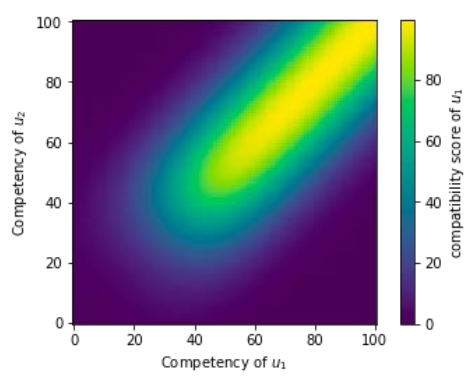
\includegraphics[width=0.4\textwidth]{g/SeekingPartnerCompatibility.PNG}
	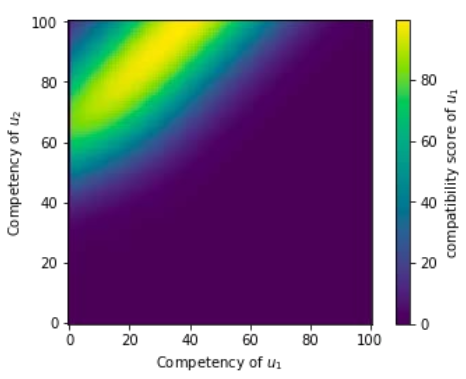
\includegraphics[width=0.4\textwidth]{g/SeekingSupportCompatibility.PNG}
	\caption{The images show the areas of compatibility of a user \(u_2\) as a function of \(u_1\)'s competency. Lighter areas mean high compatibility scores in accordance to \(u_1\)'s preferences. On the left \(u_1\) is looking for a similarly skilled study partner, leading to the best fit along the \(u_1\) = \(u_2\) axis. The cutoff beneath a competency of 40 is due to the minimum joint competency threshold \(\tau\). On the right, we can see \(u_1\) looking for peer	 support, i.e. a person with considerably higher knowledge, here about 60 points higher than \(u_1\). Source: \cite{potts2018reciprocal}}
	\label{f:Seeking}
\end{figure*}
\textit{RiPPLE} ["Recommendation in Personalised Peer Learning Environments"] was designed and developed as a web-based online learning recommendation system. \textit{RiPPLE} is an adaptive, student-facing, open-source platform with the aim to enable students to engage with others in meaningful learning experiences. To enhance the learning experience, \textit{RiPPLE} functions as a learning platform, helping students to co-create and find meaningful learning-content and to find peers to learn with. This analysis will focus on \textit{RiPPLE} as a peer recommendation platform.\\
Based on user input, \textit{RiPPLE} will calculate potential matchups for its users. Depending on
\begin{itemize}
	\item the competency derived by a user's performance on learning content
	\item his or her available time slots
	\item the topics he or she would like to provide help, seek peer support or find a learning partner in and
	\item the user's preferences on the respective skills of a potential partner in these topics.
\end{itemize}
\textit{RiPPLE} calculates a score for a matchup and will recommend a predefined amount of persons to each user. As \textit{RiPPLE} currently recommends learning opportunities for the upcoming week, updates to user preferences or competencies are represented once per week.\\
An important aspect of the recommendation algorithm is it's compatibility function, calculating a one-directional score for each combination of potential study partners, \(u_1\) and \(u_2\). In the first step, the algorithm will check whether a potential matchup is viable following two hard constraints:
\begin{enumerate}
	\item a shared time slot has to be available for both \(u_1\) and \(u_2\)
	\item the topic-specific joint competency must be greater than a predefined threshold \(\tau\). According to Blumenfeld \cite{blumenfeld1996learning}, peer learning sessions will only become effective once the learners can share a minimum understanding of the topic.
\end{enumerate}
For every pair of users satisfying these constraints, \textit{RiPPLE} will calculate their respective one-directional scores. These represent how fitting \(u_2\) is as a study partner for \(u_1\) and vice-versa. (Since the users could have defined different preferences for their competency differences, scores don't need to be symmetric.) The scores take into account how good a matchup will be in terms of overall competency level, and how the other user matches the current user's preferences. These values will be calculated across all topics relevant for \(u_1\) and \(u_2\). A visual representation of the resulting score can be seen in figure \ref{f:Seeking}.\\
These two one-directional scores could now be used to find the best partner for a specific user. To further recommend a matchup that is beneficial for both \(u_1\) and \(u_2\), the harmonic mean of both scores is considered as the "reciprocal score" of \(u_1\) and \(u_2\), a value that is now symmetric. \cite{prabhakar2017reciprocal} The harmonic mean, contrary to the arithmetic mean, pays respect to differences between it's values, making a larger gap between values less desirable. Peer-combinations with approximately similar scores will receive better final values, making matchups that are beneficial to both participants more relevant.\\
In the last step, \textit{RiPPLE} returns a predefined amount of matchups \(k\) with the best reciprocal values for each user. Although these reciprocal values are now symmetrical, the recommendations don't have to be: While from \(u_1\)'s standpoint the matchup with \(u_2\) and an (exemplary) reciprocal score of 30 could be the very best opportunity, \(u_2\) could still have a true reciprocal matchup with \(u_3\) and a value of 50.\\
For more information on \textit{RiPPLE}, the algorithm and further clarification of different variables, please refer to \cite{potts2018reciprocal}.\\	

\subsection{Evaluation}\label{paper:evaluation}
In order to test \textit{RiPPLE}'s applicability for actual use, Potts et al. designed an experimental setup in which \textit{RiPPLE} would try to propose recommendations for randomly generated test data. Specific quality measures were designed according to \cite{olakanmi2017group} to assess different fields in which \textit{RiPPLE} would have to show its capabilities. With satisfying results, \textit{RiPPLE} would be able to be used under live conditions in the course of 2018.\\
For the experimental evaluation, random data had to be generated; diverse enough to highlight edge cases but within reasonable bounds.\\ 
%For a set of 1000 users, 10 learning topics and 10 possible timeslots, each user received a random distribution of relevant values. Topic-specific competencies were expressed as a value from 0 to 100 derived from a truncated normal distribution around a random mean with fixed variance. Each user received competencies for every topic. These were then sorted from low to high, and a random number of these topics were chosen to be part of the user's request. The highest competencies of every user were classified as "providing support" roles, the lowest as "seeking support" and the median topic received a "co-study" role. In absence of empirical data, competency difference preferences were modeled as a fixed value per chosen role, as opposed to a explicitly stated preference for each user. Every "user" was made available during random timeslots.\\
To fully satisfy as a tool recommending students to one another, \textit{RiPPLE} must be able to form meaningful and successful matches for as many users as possible in reasonable time. On the other hand, minor drawbacks in the defined metrics were considered to be tolerable in this step due to the experimental and randomly generated data and some further adjustments that could be made to compensate bad values.\\
As evaluation metrics for their experimental evaluation Potts et al. decided on four values that can further be used as general Quality Measures for reciprocal recommendation algorithms:\\

\subsubsection{Scalability} \label{paper:scalability}
\begin{figure}[!t]
	\centering
	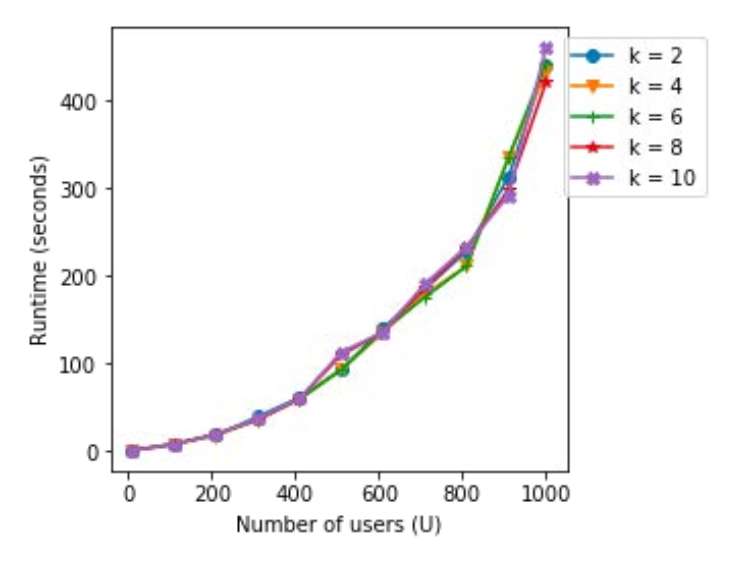
\includegraphics[width=0.4\textwidth]{g/Runtime.PNG}
	\caption{Scalability: The algorithm's runtime depending on the number of users \(U\) and the amount of recommendations per user \(k\). Note how \(k\) has almost no influence on the runtime, which grows exponentially with increasing U. Source: \cite{potts2018reciprocal}}
	\label{f:scalability}
\end{figure}
%Diese Figure ist absichtlich nicht bei der richtigen Überschrift, damit die Bilder an der richtigen Stelle im Text auftauchen. Das muss vll noch Mal gefixt werden.
\begin{figure*}[!t]
	\centering
	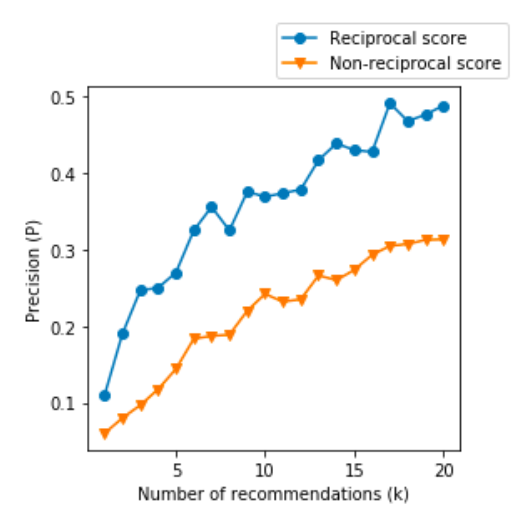
\includegraphics[width=0.4\textwidth]{g/PrecisionByK.PNG}
	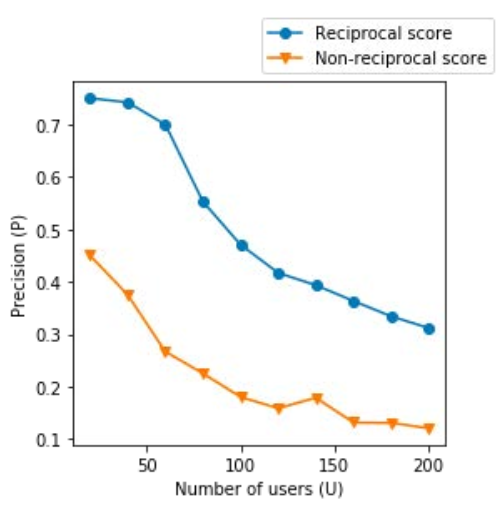
\includegraphics[width=0.4\textwidth]{g/PrecisionByU.PNG}
	\caption{Reciprocality: The precision (= the fraction of reciprocal recommendations out of the total recommendations averaged over all users) of the baseline non-reciprocal recommendations (orange) vs. of the reciprocal, averaged scores. (blue) Note how the reciprocal scores are always better. The left plot shows that increasing \(k\) also increases the precision, since more recommendations per user lead to a higher chance of reciprocal recommendations. On the right, increasing \(U\) with a fixed \(k\) reduces reciprocal precision, since there are more possible users to recommend. Source: \cite{potts2018reciprocal}}
	\label{f:reciprocality}
\end{figure*}
With increasing enrollment numbers in higher education, \textit{RiPPLE} will have to be suitable for large sets of learners. High runtime and costs for evaluating datasets with reasonable amounts of students means slower responses and a worse user experience. An optimal solution could provide immediate recommendations to any user, at any moment.\\
As can be seen in figure \ref{f:scalability}, the runtime of the algorithm increased in a quadratic fashion, as U, the total amount of users, increased: \(O(n^2)\). The number of recommendations per user however did not significantly impact the runtime. (Although the paper states that it \textit{did} in fact affect runtime, looking at the plots suggests that this might be a formatting error.)\\
Currently, \textit{RiPPLE} calculates recommendations at the end of each week for the upcoming week, making the algorithm's runtime rather unimportant. In a 1000 user experiment, \textit{RiPPLE} was able to provide recommendations for a single user in 0.045 seconds. However, further improvements are planned.\\

\subsubsection{Reciprocality} \label{paper:reciprocality}
The best social recommendations are truly reciprocal: Users contacting a recommended user would also appear on this user's list of potential study partners. \cite{prabhakar2017reciprocal} Reciprocality was tested for both, the baseline non-reciprocal and the joint reciprocal harmonic mean scores. Whenever a user appears in the recommendations of a user on their own recommendation list that was built according to the respective score, the recommendation was considered to be reciprocal.\\
The precision for every user given the used score is calculated by dividing his reciprocal recommendations through \(k\), the total amount of recommendations that user received. The system's total precision is defined as the average precision across all users. \cite{prabhakar2017reciprocal}\\ 
In all tested cases shown in figure \ref{f:reciprocality}, the reciprocal score had a higher precision than the baseline score. This is not surprising, since using the harmonic mean of both one-directional scores chooses reciprocal scores with medium values compared to non-reciprocal scores with a single high value. (As explained in section \ref{paper:RiPPLE})\\

\subsubsection{Coverage} \label{paper:coverage}
\begin{figure*}[!t]
	\centering
	\includegraphics[width=0.4\textwidth]{g/CoverageUk.PNG}
	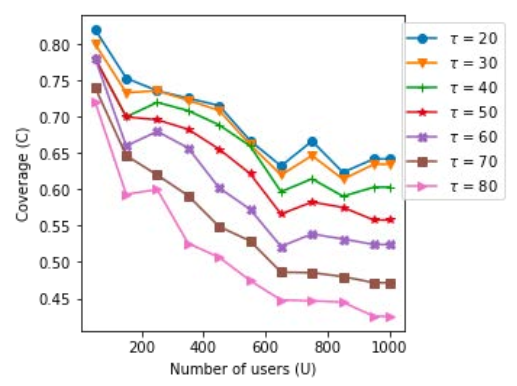
\includegraphics[width=0.4\textwidth]{g/CoverageUT.PNG}
	\caption{Coverage: The percentage of users who appear in other's recommendations. With more users, coverage sinks (likelihood of hard to match users increases). Increasing the amount of received recommendations \(k\) (left) or lowering the minimum joint competency of matches (right) increases coverage. Mind the y-axis cutoff. Source: \cite{potts2018reciprocal}}
	\label{f:coverage}
\end{figure*}
Recommending potential learning partners to one another should not abandon anyone. As such, coverage is a very important metric to consider. Since (almost) every user will receive recommendations, most users will be covered in one way or another. (The exception to this are users with completely incompatible time slots, role preferences (i.e. being the only person looking for an equally skilled study partner) or users who can't meet the minimum competency when coupled with their available potential partners.) A very good fit can only be ensured when each user is recommended to others, ideally forming a reciprocal recommendation, which is represented in metric \ref{paper:reciprocality}. Coverage however is defined as the percentage of users that appear in other's recommendations at least once.\\
For a low amount of users and lots of recommendations per user, coverage was close to 0.9, meaning most users were recommended to others. As U increased or k decreased, the coverage sunk. However, more than 40\% of users appeared in other's recommendations under all tested circumstances. Refer to figure \ref{f:coverage} for a graphical overview.\\

\subsubsection{Quality} \label{paper:quality}
\begin{figure}[!t]
	\centering
	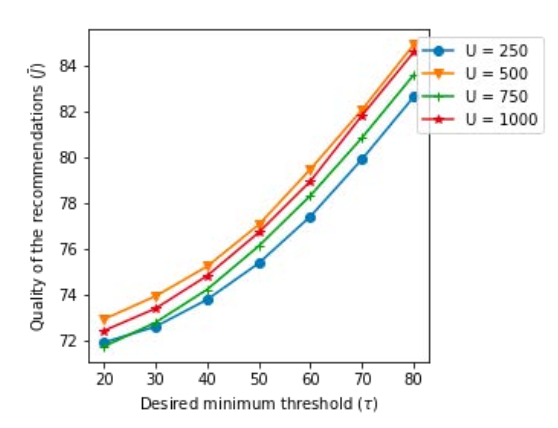
\includegraphics[width=0.4\textwidth]{g/QualityByU.PNG}
	\caption{Quality: The quality of matchups over different values for \(U\) and \(\tau\). Note how changing \(U\) does not affect matchup quality. Choosing a higher minimum joint competency threshold \(\tau\) for successful matchups increases overall quality. Note the different scaling of the axes, overemphasizing the quality increases. Source: \cite{potts2018reciprocal}}
	\label{f:quality}
\end{figure}
The quality of a recommendation is not only based on its fit, but also on how good the resulting team could perform. According to Blumenfeld, learners should meet a minimum competency level in order to be an effective group, as specified by the employed minimum matchup threshold \(\tau\). \cite{blumenfeld1996learning} Quality is thus defined as the user's average joint competencies across their matched topics. The goal is to generate matches that are as capable as possible in their respective fields of study.\\
As figure \ref{f:quality} shows, it is apparent that the total amount of users did not affect the quality of matches. The minimum threshold for joint competency of a matchup however led to a better quality. Comparing this finding to figure \ref{f:coverage} however, suggests that higher quality comes at the cost of less coverage. Especially when considering the slight improvements in quality score for larger increments in \(\tau\).\\

\section{Discussion} \label{extensions}
Reciprocal peer recommendation is a highly promising topic with lots of applications, but is hard to handle, as a closer examination of "Reciprocal peer recommendation for Learning Purposes" and the implemented platform \textit{RiPPLE} have shown. The system introduced by Potts et al. presents an approach to build a scalable, interactive and user-facing multi-purpose platform to enhance learning both in on- and offline circumstances.\\
The preliminary experimental evaluation of the platform's performance using artificial data sheds light on variable relationships, potential initial values for scientifically sparse concepts and the interplay of lots of factors. While the reported values present good metrics to measure the algorithm's performance and suitability for live data, they don't actually evaluate the algorithm, since no real data was considered and no target values have been set. Although the data is quantifiable, these findings should not be mistaken as quantitative results: instead of comparing the data to theory-driven goals and evaluating them for actual use, they are more or less providing an overview of how the algorithm works. In fact, there is currently no way to know if these results are "good". Some of the used measurements lack consistent data and research, and are not theoretically funded. For example, the question whether a coverage of little above 0.4 will be enough in practice, remains unanswered. Actual results from live usage are thus highly interesting and could provide insights in lots of different areas. The importance of user-centered on top of systemic evaluations has been discussed in several studies, specifically user satisfaction information might not be congruent with data-centric findings. \cite{7994718, olakanmi2017group}\\
\textit{RiPPLE} is concerned with theoretical criticisms regarding social learning RS research, and Potts et al. tried to pay respect to many problems. Summarizing many of these issues, a highly influential report by Olakanmi and Vassileva \cite{olakanmi2017group} highlights common shortcomings of peer recommendation studies and their proposed systems:
\begin{itemize}
	\item Focus on improving learning instead of the goals of learning
	\item No information regarding the collection of user data
	\item Randomly assigning users in the first iteration and improving based on findings
	\item No consideration of scalability of the algorithm
	\item Inflexibility in working with fixed and limited constraints
	\item Too detailed user models leading to impossible matching
	\item Inflexibility in dealing with only partially known users
	\item Usage of self-reported user preference data
	\item Orphaned learners don't receive any value and have to be processed by hand
	\item No valid evaluation, just providing proofs of concept
\end{itemize}
\textit{RiPPLE} was obviously built with these criticisms in mind, and tried to improve on the basis of earlier algorithms. For example, \textit{RiPPLE} aims to provide actual benefits to learners, uses a detailed user model and assigns students as informed as possible. Scalability and many other factors were considered when reporting the platform's theoretical applicability in section \ref{paper:evaluation}. \textit{RiPPLE}'s flexibility in the definition of threshold values allows the tool to be customized to specific scenarios and needs.\\ 
However, many of the criticisms remain problematic until disproven: \textit{RiPPLE}'s user model is light-weight but not evaluated and rather rigid, relying on the user's motivation to self-report data. The algorithm allows for learners to be orphaned due to different situations (as described below). Finally, as has already been stated, \textit{RiPPLE} has not yet been evaluated in a real scenario.\\
Besides all this theoretical criticism, the algorithm itself does have some practical drawbacks as well. For one, \textit{RiPPLE} calculates matchups across all topics. For example, two learners who would be a perfect match in one topic, but a bad match in another would be considered as a mediocre match. Topic-wise recommendation could further complicate the algorithm, but might lead to larger benefits for users.\\
Another way to improve the overall utility would be to consider slightly larger groups instead of matchups of two. Lots of theory about group composition emphasizes the importance of different skillsets and heterogeneity. \cite{olakanmi2017group, blumenfeld1996learning, manske2015using} A system called DIANA, using a genetic framework to form small heterogeneous groups in study courses used many different student characteristics to match students. An evaluation using course grades proved that this could generally be more efficient than random or self-organized group formation. \cite{moreno2012genetic}\\
Another problem of \textit{RiPPLE} are edge-cases in terms of competency preferences that would lead to overall low scores for matchups with other people, leading to learners who will receive suggestions with low scores, but won't appear in other's recommendations. While this does not necessarily lead to any consequences by itself, certain highly compatible users might be overwhelmed with meeting-requests from users outside their own recommendations. While they won't be able to meet every requesting user, these less compatible users might become abandoned.\\
Another drawback is the neglected human factor. Both user buy-in and competence in handling the tool and its demands might influence its use in practice. While this study's explicit goal was to only test the theory and future praxis tests are planned, this topic should still be discussed, a major shortcoming of the paper at hand.\\
A lack in user buy-in is something that should always be considered, especially in a student context. If a student didn't want to engage with strangers, was not motivated to study with partners or to adjust his or her schedule, all recommendations to and of that student would not accomplish anything. Meeting requests would be ignored, and opportunities for matchups would expire. Even negative user manipulation needs to be considered as a possibility, but is something that has to be dealt with in the live test.\\
While missed opportunities are a problem of the students themselves, rather than of the platform providing recommendations, the other human factor needs to be addressed directly by the tool:\\
As humans are unreliable, self-reported metrics always underly lots of variance and errors. A user's competency in a specific topic, his or her preferences, or the willingness to commit to a specific timeslot for learning might change daily, depending on mood, time of day, culture and lots of other factors. \cite{lee2002cultural} \cite{sorensen2008measuring} Other variables, like a user's preferred skill difference towards a learning partner, are especially hard to specify. How is a user supposed to know what his or her learning preferences are? How would he know which number refers to the desired difference in skill rating? From a psychological standpoint, this operationalization is bound to fail, if not controlled in an appropriate manner. \cite{gonyea2005self}\\
This whole issue is not solely a problem of "Reciprocal peer recommendation for Learning Purposes". Generally speaking, choosing a user preference model that fits both the domain and the goal of an algorithm while still being able to perform in praxis poses a major problem in peer recommendation. \cite{potts2018reciprocal, olakanmi2017group} In reciprocal recommendation, this issue becomes even more prevalent, since the user must be modeled as both, a recommended item and a user receiving recommendations at the same time.\\
An important factor is to consider both, the information needed to create meaningful matches according to a specific success criterion, and how to access this information. Usually, automatically collected data is preferred to relieve the users as much as possible. But not all data can automatically be collected. Internal information, like preferences, date availability, motivations or the highly important factor of personality need to be reported by the user - there is currently no way to easily access internal information of the user's mind.\\
Psychological research was founded to enable the measurement and quantification of these details. From psychophysical measurements to intricate operationalizations of complicated internal states, one easily accessible method stays predominant in social science: self-reported statements, from qualitative interviews to acceptance scales.\\
One such scale is the NEO-PI-R \cite{ostendorf2004neo}, arguably one of the most famous personality-measurement tools. A questionnaire with Likert-scaled \footnote{The commonly known items prompting users to reply to a statement on a scale from (usually) 1 to 5 (often combined with sentences like "I agree" or "I disagree") are called "Likert scales" after Rensis Likert. \cite{likert1932technique}} items on five axes representing the five dimensions of personality. \cite{mccrae1987validation, goldberg1990alternative}\\
While the NEO-PI-R is widely used and considered as reliable and validated, it still relies on self- or peer-reported data and can, as such, not be considered a flawless tool. For example, many self-reporting tools suffer from a relevant problem called "Faking Good", the tendency to answer items in a way that is considered to be socially acceptable. When faking good, people manipulate their answers to cohere to social norms out of fear to be seen as a bad person. "Faking Good" is known to influence the outcomes of some personality traits measured by the NEO-PI-R.\cite{griffin2004applicants} A similar effect can be observed when peer-ratings get influenced by peer sympathy. \cite{leising2010letter}\\
In learning environments, a phenomenon known as the "Lake Wobegon Effect" influences student reports of their learning success: students tend to overstate their good performances, while failures will not be reported. This leads to an overestimation of student successes in surveys. \cite{maxwell1994lake}\\
As another example, the infamous "Likert Scale" as introduced by Rensis Likert in 1932 as an "attitude scale" \cite{likert1932technique} can safely be assumed to be one of the most used metrics in social research, while it's optimal use still remains questionable. \cite{chang1994psychometric, lee2002cultural}\\
Self-reported data is a largely controversial topic in psychological research: it is easy to acquire and enables researchers to access internal information, while these measurements can fluctuate following lots of different influences and are hard to validate. \cite{gonyea2005self, lee2002cultural, sorensen2008measuring}\\
In summary, modeling users is complicated due to unreliable methods or participants (knowingly or subconsciously) manipulating their answers.\\
While Potts et al. obviously tried to choose a user-model that is limited to the necessary basics and tried to rely on as few ambiguous and self-reported pieces of information as possible, they \textit{still} need a user's ability in reporting information about him- or herself.\\
Other reciprocal recommendation approaches have to work around the same problems. As mentioned in section \ref{rw:reciprocalrec}, Xia et al. have shown that a behavior-emergent metric was more reliable in their use case of reciprocal online-dating recommendation. \cite{xia2014characterization} Instead of focusing on user-reported data alone, they included implicit and pre-evaluated information derived from user interactions to measure attractiveness and willingness to communicate. \cite{xia2015reciprocal} Wang et al. wanted to improve gaming matchmaking by employing problem-solving style information gathered from in-game statistics. They were able to deduce complicated, high-level cognitive problem-solving skills from simply evaluating implicit behavior, and used this information to improve player experiences. \cite{wang2015thinking}\\
Instead of asking learners for their preferences regarding the competency difference towards their peer, Potts et al. could have decided on values founded in theory of optimal group composition. \cite{manske2015using}\\
The contrary approach of data collection is to  use implicit data derived from a user's interaction with the running system. An important drawback to this method, mentioned by Olakanmi et al., needs to be considered: the cold start problem. \cite{olakanmi2017group} Relying on live data will lead to the first recommendations to be made without any underlying data, at random. Only after some burn-in, actual data can be used to achieve better results, which leads to much less initial acceptance for the new tool.\\
Another drawback of implicit data is finding a correct operationalization of relevant variables. As shown in section \ref{rw:usermodeling}, systems in a straightforward domain such as gaming matchmaking can choose many completely different approaches to measure good experiences and fair matches for players. An approach valid in one situation might be completely ill fitting after changing the game, genre, game mode, users or goal of the RS. Finding viable measurements that are reliable and valid is one of the major concerns of psychological experimental design. Implicit data might be more reliable, but is hard to design.\\
But what kind of data is better for any given Recommender System? The discussion about implicit versus explicit data acquisition and user feedback is still ongoing. As has been established in the former paragraphs, while explicit data is easy to collect but often biased by subjective inabilities to properly report it, implicit data is more objective but harder to acquire, especially for some specific bits of data.\\
In another recent study, fittingly named "Explicit or Implicit Feedback? [...]" \cite{zhao2018explicit}, Zhao et al. compared different recommendation algorithms in different performance criteria. They collected implicit (user interactions with the recommended items) and explicit (user feedback) information, but used different subsets for training their RSs. Their main finding was that machine-learning algorithms optimized on implicit action prediction led to higher engagement results from users. Systems learning with explicit user feedback however, led to more user satisfaction in comparison. Unsurprisingly, the system maximized what it was told to maximize. However, users were more satisfied with a system that was not concerned with engagement rates, but with overall quality, even if this might incorporate less interactions. The authors conclude that this might have contributed to late research focusing on implicit feedback and neglecting the actual benefit for a user while focusing on the higher engagement rates, which include both negative and positive interactions. While still lots of studies focus primarily on systemic data instead of actually testing their prototypes with users \cite{7994718}, an interaction between the endorsement of high engagement rates and low evaluation expenses emerges. However, as Zhao et al.'s work confirms, explicit user feedback is still considered to be highly important to actually monitor user satisfaction and system performance. \cite{BUDER2012207, 7994718}\\
The last and probably most important finding of Zhao et al.'s work was that a combined data approach worked even better: implicit and explicit data taken together can often outperform regular systems. As other research confirmed, checking for user's feelings about a recommendation and validating it by watching implicit data delivers more reliable data than any singular approach could. \cite{zhao2018explicit, 8328917,7994718}\\

\section{Conclusion}
As no truly satisfying approach to choose data and models for effective group formation in a new and untouched cohort of peers has yet been found, Potts et al. struggle to compile a convincing user model themselves. They incorporated explicit and implicit user data into their system, but could not avoid all of the pitfalls of data collection.\\ 
Taking all of this into consideration, their proposed peer learner recommendation algorithm does have its flaws but could still benefit learners in praxis. Reciprocally matching students according to their needs and preferences is likely to help at least some students achieve better grades and form new social connections.\\
The applications of reciprocal peer recommendation are manifold and generally beneficial in a highly social and connected modern world. Bringing different people together and providing opportunities to engage with one another yields many advantages and teaches meaningful skills. However, human factors need to be incorporated in the algorithms to account for the dualistic role of users as both recommended items and recipients of recommendations. Many experiments with explicitly and implicitly collected data have uncovered a vast array of issues that need to be navigated. Especially due to the many problems associated with measuring humans, algorithms are still unreliable when handling people in reciprocal situations. However, skillful design can circumvent some of these problems and create systems that are far from perfect, but nonetheless beneficial to their users. Time will tell if \textit{RiPPLE's} streamlined user model and up-front evaluation of technical measures have made it a platform fit for practical use. Until then, further research is required.\\

% An example of a floating figure using the graphicx package.
% Note that \label must occur AFTER (or within) \caption.
% For figures, \caption should occur after the \includegraphics.
% Note that IEEEtran v1.7 and later has special internal code that
% is designed to preserve the operation of \label within \caption
% even when the captionsoff option is in effect. However, because
% of issues like this, it may be the safest practice to put all your
% \label just after \caption rather than within \caption{}.
%
% Reminder: the "draftcls" or "draftclsnofoot", not "draft", class
% option should be used if it is desired that the figures are to be
% displayed while in draft mode.
%
%\begin{figure}[!t]
%\centering
%\includegraphics[width=2.5in]{myfigure}
% where an .eps filename suffix will be assumed under latex, 
% and a .pdf suffix will be assumed for pdflatex; or what has been declared
% via \DeclareGraphicsExtensions.
%\caption{Simulation results for the network.}
%\label{fig_sim}
%\end{figure}

% Note that the IEEE typically puts floats only at the top, even when this
% results in a large percentage of a column being occupied by floats.


% An example of a double column floating figure using two subfigures.
% (The subfig.sty package must be loaded for this to work.)
% The subfigure \label commands are set within each subfloat command,
% and the \label for the overall figure must come after \caption.
% \hfil is used as a separator to get equal spacing.
% Watch out that the combined width of all the subfigures on a 
% line do not exceed the text width or a line break will occur.
%
%\begin{figure*}[!t]
%\centering
%\subfloat[Case I]{\includegraphics[width=2.5in]{box}%
%\label{fig_first_case}}
%\hfil
%\subfloat[Case II]{\includegraphics[width=2.5in]{box}%
%\label{fig_second_case}}
%\caption{Simulation results for the network.}
%\label{fig_sim}
%\end{figure*}
%
% Note that often IEEE papers with subfigures do not employ subfigure
% captions (using the optional argument to \subfloat[]), but instead will
% reference/describe all of them (a), (b), etc., within the main caption.
% Be aware that for subfig.sty to generate the (a), (b), etc., subfigure
% labels, the optional argument to \subfloat must be present. If a
% subcaption is not desired, just leave its contents blank,
% e.g., \subfloat[].


% An example of a floating table. Note that, for IEEE style tables, the
% \caption command should come BEFORE the table and, given that table
% captions serve much like titles, are usually capitalized except for words
% such as a, an, and, as, at, but, by, for, in, nor, of, on, or, the, to
% and up, which are usually not capitalized unless they are the first or
% last word of the caption. Table text will default to \footnotesize as
% the IEEE normally uses this smaller font for tables.
% The \label must come after \caption as always.
%
%\begin{table}[!t]
%% increase table row spacing, adjust to taste
%\renewcommand{\arraystretch}{1.3}
% if using array.sty, it might be a good idea to tweak the value of
% \extrarowheight as needed to properly center the text within the cells
%\caption{An Example of a Table}
%\label{table_example}
%\centering
%% Some packages, such as MDW tools, offer better commands for making tables
%% than the plain LaTeX2e tabular which is used here.
%\begin{tabular}{|c||c|}
%\hline
%One & Two\\
%\hline
%Three & Four\\
%\hline
%\end{tabular}
%\end{table}


% Note that the IEEE does not put floats in the very first column
% - or typically anywhere on the first page for that matter. Also,
% in-text middle ("here") positioning is typically not used, but it
% is allowed and encouraged for Computer Society conferences (but
% not Computer Society journals). Most IEEE journals/conferences use
% top floats exclusively. 
% Note that, LaTeX2e, unlike IEEE journals/conferences, places
% footnotes above bottom floats. This can be corrected via the
% \fnbelowfloat command of the stfloats package.


% references section

% trigger a \newpage just before the given reference
% number - used to balance the columns on the last page
% adjust value as needed - may need to be readjusted if
% the document is modified later
%\IEEEtriggeratref{8}
% The "triggered" command can be changed if desired:
%\IEEEtriggercmd{\enlargethispage{-5in}}


\bibliographystyle{IEEEtran}
\bibliography{bib}

% that's all folks
\end{document}


